\let\textcircled=\pgftextcircled
\chapter{Utilising the Kalman Filter}
\label{chap:utilisingkalman}

\initial{T}he Kalman filter described in chapter \ref{chap:introkalmanfilter} is clearly a very basic model dealing with only one dimension. In the reality of this project though, the drone will have to work in relation to a three dimensional world. This means that the filter will need to be expanded to reflect these additional dimensions, as well as take in and provide any additional data deemed necessary for operation of the drone's systems. \par

\section{Expanding to Three Dimensional Movement}
With one dimension the simplistic state contained only two items, position and velocity. Three dimensional position and velocity will require more items for each, however there are a number of different ways to represent them \cite{windall2008other}.

\subsection{Three Dimensional Position}
There are three main positional coordinate systems; Cartesian, cylindrical and spherical.
\begin{itemize}
\item Cartesian coordinates use the classic orthogonal axes, for three dimensions this requires three axes usually denoted x, y and z.
\item Cylindrical coordinates use a single axis (usually denoted z), and then specify a location in space by giving a radial angle (\(\Theta\)) and a distance from a point along the axis (r) as exampled in figure \ref{fig:cylindricalcoordinates}.

\begin{figure}[t!]
	\centering
	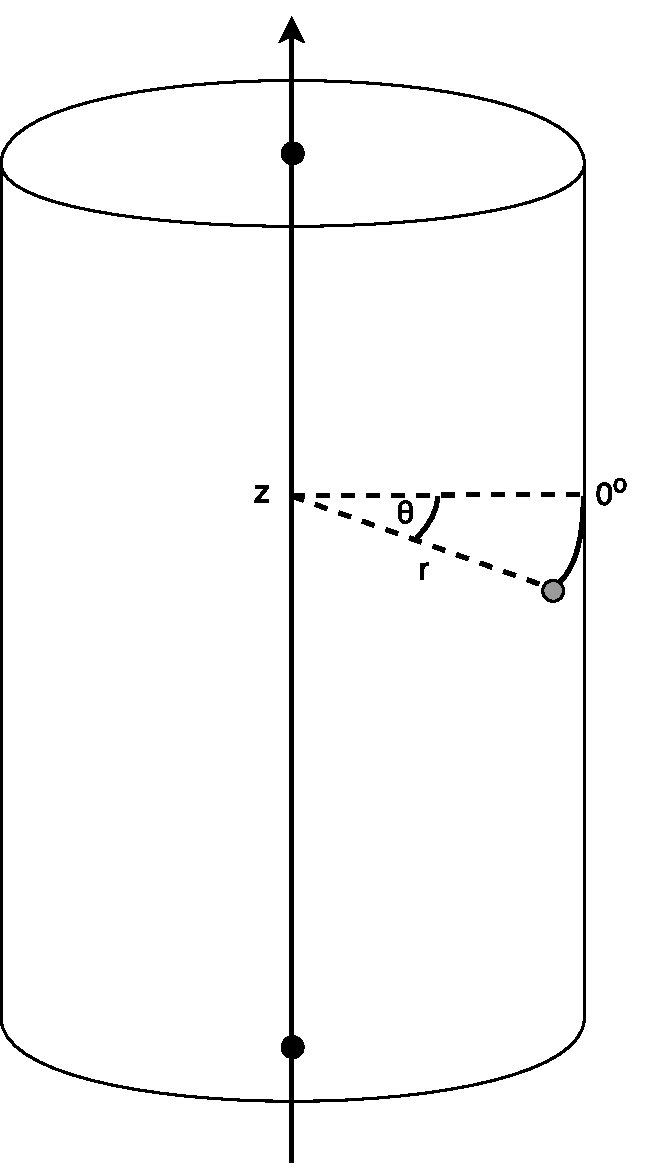
\includegraphics[height=0.45\textheight]{cylindrical.pdf}
	\mycaption[Cylindrical Coordinates Diagram]{Diagram showing the workings of cylindrical coordinates.}
	\label{fig:cylindricalcoordinates}
\end{figure}

\item Spherical coordinates require a polar axis and a perpendicular plane. The spatial position is then given by an angle around the plane (azimuth), an angle perpendicular to the plane (elevation) and a distance from the origin.
%^diagram spherical coordinates
\end{itemize}

As can be seen, all three systems require three state items to represent a spatial location. Since Cartesian coordinates are those most widely understood and with no obvious drawbacks when compared with the other systems, it seems to make sense that they should be used.

\subsection{Three Dimensional Velocity}
Velocity description is very similar to positional, although the cylindrical system is more complicated to visualise in this instance.
\begin{itemize}
\item The Cartesian system uses the three axes to describe movement relative to each orthogonal direction. These three combined give a single velocity vector.
\item In the cylindrical system movement along the single axis is easy to visualise, being identical to one of the axes in the Cartesian system. The equivalent of the other two axes however is a function of both the change in radial angle and distance from the central axis.
\item The spherical coordinate system in contrast is very intuitive. The origin is thought of as the moving object, the azimuth and elevation describe the movement direction, and the distance from the origin is instead the absolute velocity.
\end{itemize}

Although the spherical coordinate system is an elegant and intuitive system, the Cartesian system was chosen to match the positional one so as to avoid confusion and to make kinematic equations more simple to apply.

\subsection{Three Dimensional Orientation}
Several of the other systems on the drone require accurate orientation data to function. To this end including orientation was seen to be a natural step due to the importance of the information and the multiple inertial measurement units that will be available to provide the relevant data. Again there are a number of coordinate systems available, though these are more or less identical to the velocity systems, albeit with the absolute velocity component being unimportant. This has bigger ramifications than might be expected. The spherical and cylindrical systems used above are known as the quaternion system when related to orientation and have a couple of large benefits \cite{grossekatthofer2012introduction}\cite{grassia1998practical}.
\begin{itemize}
\item In the previous systems there is a  component relating to distance or absolute velocity. In the quaternion representation this is wholly unnecessary and can be removed. This reduces the number of state items required to two when compared to the three the other systems use.
\item The Cartesian system experiences a phenomenon known as gimbal lock when two of the axes occupy the same plane, effectively leading to a loss of orthogonality. This causes a loss of one of the three degrees of freedom. The quaternion system does not suffer from this effect.
\end{itemize}

Once again, the Cartesian system was chosen since it fits mathematically into the existing framework more easily. Additionally, drones do not pitch at close to 90\textsuperscript{o} under normal operating conditions so the issue of gimbal lock should not occur.
























